%------------------------------------------------------------------------------
%  Data Processing -- Master in Telecommunication Engineering, UC3M
%  Deep Learning block: three sessions
%  Compile with:  latexmk -xelatex deeplearning.tex   (pdflatex also works)
%------------------------------------------------------------------------------
\documentclass[aspectratio=169,10pt]{beamer}
\usetheme{metropolis}

\usepackage{iftex}
\ifXeTeX
  \usepackage{fontspec}
  \IfFontExistsTF{Fira Sans}{%
    \setsansfont{Fira Sans}[Numbers=Lining]%
    \setmonofont{Fira Mono}[Scale=MatchLowercase]%
  }{}
\fi
\usepackage{amsmath,amssymb,bm}
\usepackage{booktabs}
\usepackage{graphicx}
\usepackage{tikz}
\usepackage{listings}
\usepackage[most]{tcolorbox}

%--------------------------------------------------------------- house colours
\definecolor{uc3m}{RGB}{0,53,120}
\definecolor{accent}{RGB}{224,118,27}
\definecolor{okgreen}{RGB}{60,141,90}
\definecolor{lightgrey}{RGB}{242,242,242}

\setbeamercolor{frametitle}{bg=uc3m, fg=white}
\setbeamercolor{title separator}{fg=accent}
\setbeamercolor{progress bar}{fg=accent}
\setbeamercolor{alerted text}{fg=accent}
\setbeamercolor{example text}{fg=okgreen}
\setbeamercolor{section title}{fg=uc3m}
\setbeamercolor{block title}{bg=lightgrey, fg=uc3m}

\metroset{block=fill, sectionpage=progressbar, numbering=fraction}

%--------------------------------------------------------------- code listings
\lstset{language=Python,
        basicstyle=\ttfamily\scriptsize,
        keywordstyle=\color{uc3m}\bfseries,
        commentstyle=\color{gray}\itshape,
        stringstyle=\color{okgreen},
        showstringspaces=false,
        breaklines=true,
        columns=fullflexible,
        keepspaces=true,
        aboveskip=.4em, belowskip=.2em}

%--------------------------------------------------------------- helper macros
\newcommand{\vx}{{\bm x}}
\newcommand{\vy}{{\bm y}}
\newcommand{\vw}{{\bm w}}
\newcommand{\vW}{{\bm W}}
\newcommand{\vb}{{\bm b}}
\newcommand{\vh}{{\bm h}}
\newcommand{\vq}{{\bm q}}
\newcommand{\vo}{{\bm o}}

% Tag shown on the section pages. Must be renewed BEFORE \section
\newcommand{\sessiontag}{}
\setbeamertemplate{section page}{%
  \begin{center}
    {\usebeamerfont{section title}\usebeamercolor[fg]{section title}%
     \scshape\small \sessiontag \par}
    \vspace{.6em}
    {\usebeamerfont{section title}\usebeamercolor[fg]{section title}%
     \Large\insertsectionhead\par}
  \end{center}}

% "Now you" practice block
\newtcolorbox{practice}[1][]{%
  enhanced, breakable, colback=accent!6, colframe=accent,
  boxrule=.8pt, left=2mm, right=2mm, top=1.2mm, bottom=1.2mm,
  fonttitle=\bfseries, coltitle=white, colbacktitle=accent,
  title={#1}}

\newtcolorbox{keybox}[1][]{%
  enhanced, colback=uc3m!5, colframe=uc3m, boxrule=.8pt,
  left=2mm, right=2mm, top=1.2mm, bottom=1.2mm,
  fonttitle=\bfseries, coltitle=white, colbacktitle=uc3m, title={#1}}

\newtcolorbox{warnbox}[1][]{%
  enhanced, colback=accent!5, colframe=accent!80!black, boxrule=.8pt,
  left=2mm, right=2mm, top=1.2mm, bottom=1.2mm,
  fonttitle=\bfseries, coltitle=white, colbacktitle=accent!80!black, title={#1}}

\title{Deep Learning}
%\subtitle{Neural networks, PyTorch and convolutional networks}
\author{Jerónimo Arenas García \\ Data Processing \\ Master in Telecommunication Engineering}
\institute{Universidad Carlos III de Madrid}
%\date{2026--27}
\date{}
\begin{document}

{\setbeamercolor{background canvas}{bg=white}
\maketitle}

%==============================================================================
\begin{frame}[t]{Outline}
\begin{columns}[T]
\begin{column}{.62\textwidth}
\begin{enumerate}
  \item \textbf{Neural networks from scratch}\\
        {\small Everything with numpy: topology, loss, forward, \alert{backward},
         gradient descent.}\\[.2em]
        {\footnotesize\ttfamily DL1\_NeuralNetworks\_numpy.ipynb}
  \item \textbf{Deep networks with PyTorch}\\
        {\small The same models with a library that computes the gradients,
         plus optimization and generalization.}\\[.2em]
        {\footnotesize\ttfamily DL2\_DeepNetworks\_PyTorch.ipynb}
  \item \textbf{Convolutional networks}\\
        {\small A topology designed for images, data augmentation and
         transfer learning.}\\[.2em]
        {\footnotesize\ttfamily DL3\_ConvolutionalNetworks.ipynb}
\end{enumerate}
\vspace{-.6em}
\end{column}
\begin{column}{.36\textwidth}
\begin{keybox}[How these sessions work]
\small
\begin{itemize}
    \item Short blocks of theory, then you work on the notebook.
    \item All notebooks run in Google Colab with GPU.
    \item Local deployments need to install PyTorch.
\end{itemize}

\end{keybox}
\end{column}
\end{columns}
\end{frame}

%==============================================================================
\renewcommand{\sessiontag}{Session 1 \textbullet{} notebook DL1}
\section{Neural networks from scratch}

\begin{frame}{Why now?}
Feed-forward neural networks have been around since the 1960s, but only in the last
10--15 years have they met their expectations.

\begin{columns}[T]
\begin{column}{.5\textwidth}
\begin{itemize}
  \item Computation at scale (GPUs, cloud)
  \item Very large datasets
  \item Topologies suited to particular problems\\(CNNs, RNNs, Transformers)
  \item Training strategies that generalize better
\end{itemize}
\end{column}
\begin{column}{.46\textwidth}
\begin{keybox}[You already know SLPs]
\small
We start from something you already know: \alert{logistic regression}.

A single-layer network with logistic activation and cross-entropy loss \emph{is}
logistic regression.
\end{keybox}
\end{column}
\end{columns}
\end{frame}

\begin{frame}{The two datasets}
\begin{columns}[T]
\begin{column}{.48\textwidth}
\textbf{Sign language digits}
\begin{itemize}\small
  \item 2062 images, $64\times64$, grayscale
  \item 10 classes, one-hot encoded
  \item Also used as a binary problem (digits 0 vs 1)
\end{itemize}
\end{column}
\begin{column}{.48\textwidth}
\textbf{Dogs vs Cats}
\begin{itemize}\small
  \item 25000 images, resized to $64\times64$, grayscale
  \item Binary problem
\end{itemize}
\end{column}
\end{columns}
\vspace{1em}
In both cases the image is \textbf{flattened} into a vector of $64\times64=4096$ features.

\begin{warnbox}[Keep this in mind all session]
Flattening throws away the fact that neighbouring pixels are related. Everything we do
until session 3 ignores the structure of the image. The accuracy we get on Dogs vs Cats
will remind us of that.
\end{warnbox}
\end{frame}

%------------------------------------------------------------------ single layer
\begin{frame}{A single-layer network for binary classification}
\begin{columns}[T]
\begin{column}{.55\textwidth}
\centering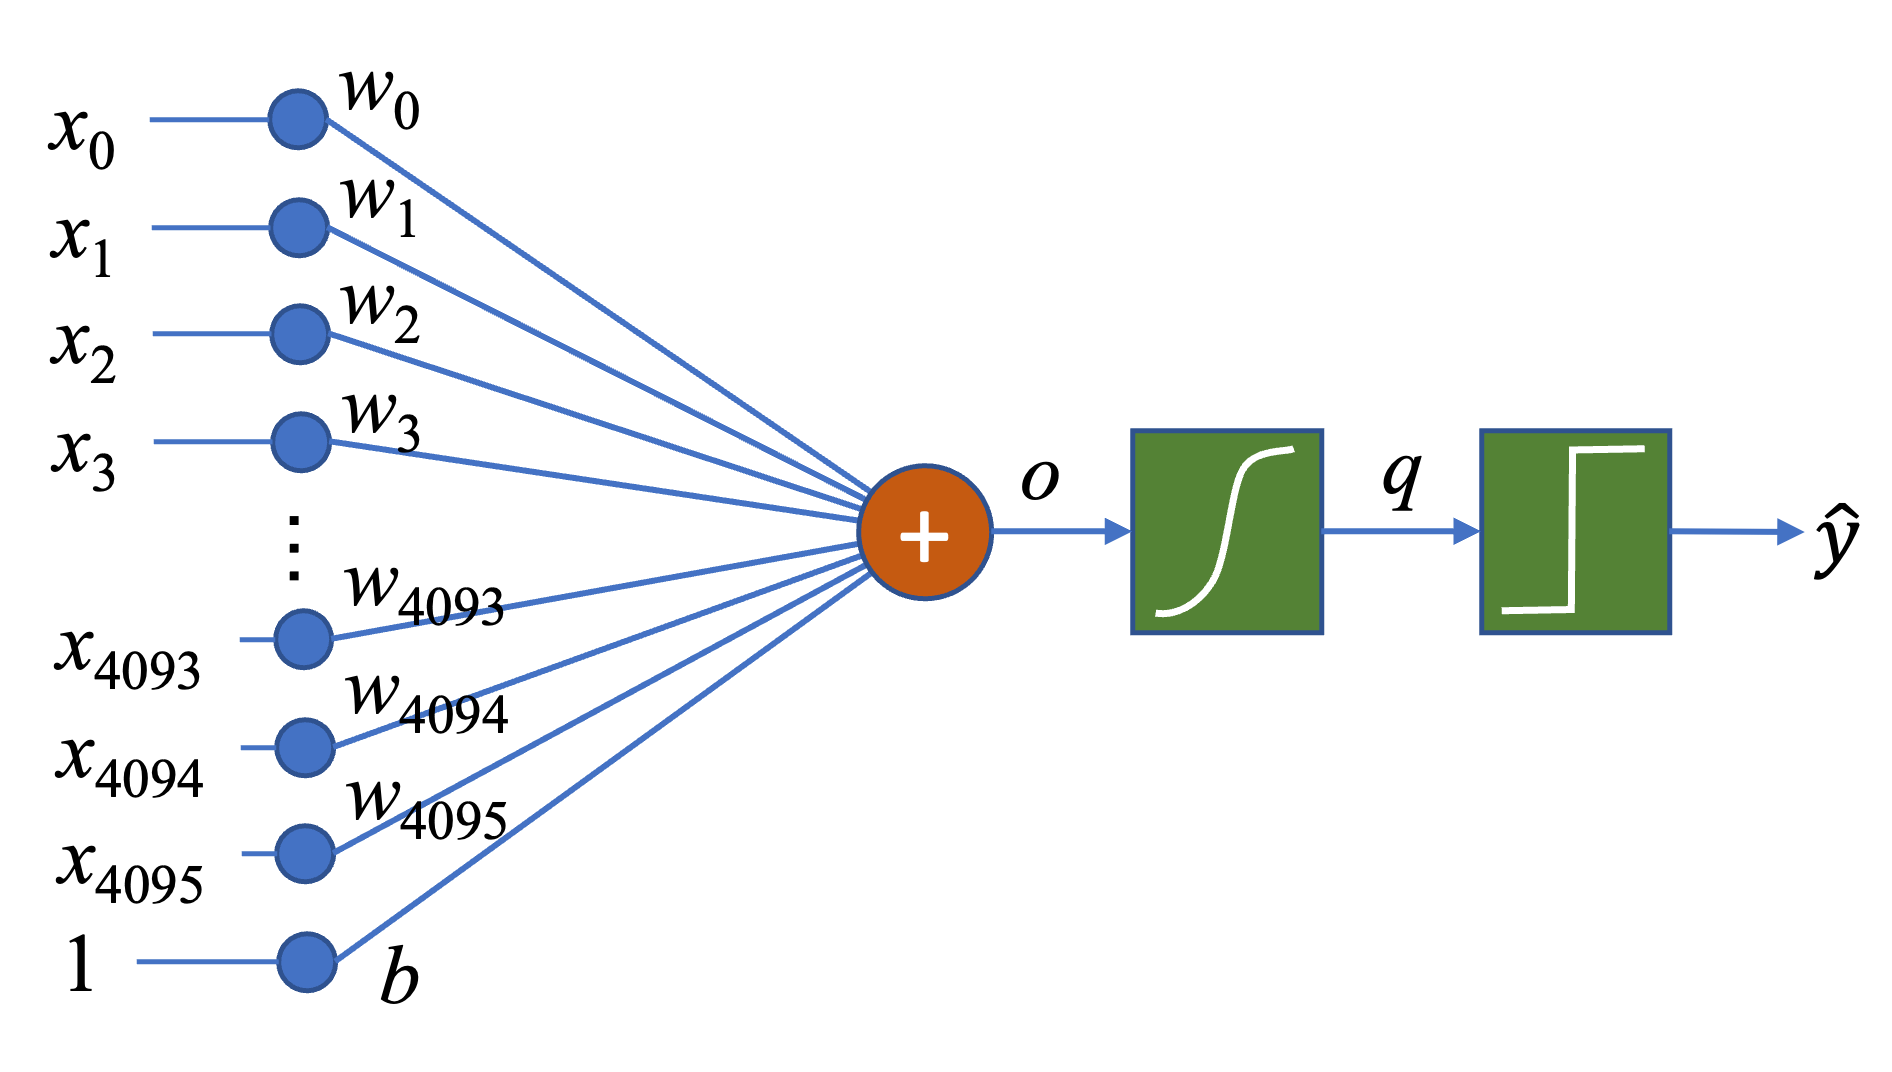
\includegraphics[width=\linewidth]{figs/LR_network.png}
\end{column}
\begin{column}{.43\textwidth}
\begin{enumerate}\small
  \item \textbf{Linear combination}
        $$o = \vw^\intercal \vx + b$$
  \item \textbf{Activation}, bounded range
        $$q = g(o) = \frac{1}{1+e^{-o}}$$
  \item \textbf{Threshold}, the hard decision
        $$\hat y = \mathbb{I}~[q \ge \tfrac12]$$
\end{enumerate}
\end{column}
\end{columns}
\end{frame}

\begin{frame}{We cannot train on the accuracy}
The accuracy is what we care about, but it is useless as a training criterion: the
threshold is not differentiable, and its derivative is zero everywhere else.

We need a \alert{loss}, a differentiable measure of disagreement between $y$ and $q$:
\begin{itemize}
  \item Square error: $\ell_2(y,q) = (y-q)^2$
  \item Absolute error: $\ell_1(y,q) = |y-q|$
  \item \alert{Cross entropy}: $\ell_\text{CE}(y,q) = -y\log q - (1-y)\log(1-q)$
\end{itemize}
and we minimize the \textbf{empirical risk} $R(\vw,b) = \sum_k \ell(y_k,q_k)$.
\end{frame}

\begin{frame}{This is logistic regression}
A network with probabilistic outputs defines a probability model:
$$P(y=1\mid \vw,b,\vx) = g(\vw^\intercal\vx + b)$$

\begin{align*}
\text{NLL}(\vw,b) &= -\sum_k \log P(y_k\mid \vw,b,\vx_k) \\
                 &= -\sum_k \big(y_k\log q_k + (1-y_k)\log(1-q_k)\big)
                  = \sum_k \ell_\text{CE}(y_k,q_k)
\end{align*}

\begin{keybox}[The point]
Minimizing the cross entropy \emph{is} maximum likelihood. Everything you know about
logistic regression carries over; what is new is that we are about to stack these units.
\end{keybox}
\end{frame}

\begin{frame}{Training: gradient descent}
Chain rule, one step at a time:
$$\frac{\partial \text{NLL}}{\partial \vw}
  = \underbrace{\frac{\partial \text{NLL}}{\partial q}}_{\frac{1-y}{1-q}-\frac{y}{q}}
    \cdot \underbrace{\frac{\partial q}{\partial o}}_{q(1-q)}
    \cdot \underbrace{\frac{\partial o}{\partial \vw}}_{\vx}
  = \sum_k (q_k - y_k)\,\vx_k$$

so the learning rules are remarkably simple:
$$\vw_{n+1} = \vw_n + \rho_n \sum_k (y_k - q_{k,n})\,\vx_k $$ 
$$b_{n+1} = b_n + \rho_n \sum_k (y_k - q_{k,n})$$

\begin{center}\small
\alert{error $\times$ input}: this shape will come back in every layer of every network.
\end{center}
\end{frame}

\begin{frame}[fragile]{Four functions, and that is the whole network}
\begin{columns}[T]
\begin{column}{.5\textwidth}
\begin{lstlisting}
def forward(w, b, x):
    return logistic(x @ w + b)

def loss(y, q):
    return -(y @ np.log(q)
             + (1-y) @ np.log(1-q)) / len(y)

def backward(y, q, x):
    w_grad = x.T @ (q - y) / len(y)
    b_grad = np.mean(q - y)
    return w_grad, b_grad

def accuracy(y, q):
    return np.mean(y == (q >= 0.5))
\end{lstlisting}
\end{column}
\begin{column}{.46\textwidth}
\begin{keybox}[Anatomy of any network]
\small
\begin{itemize}
  \item topology \;$\rightarrow$\; \texttt{forward}
  \item criterion \;$\rightarrow$\; \texttt{loss}
  \item gradients \;$\rightarrow$\; \texttt{backward}
  \item update rule \;$\rightarrow$\; the training loop
\end{itemize}
Only \texttt{backward} will become hard. In session 2 we will stop writing it.
\end{keybox}
\end{column}
\end{columns}
\end{frame}

\begin{frame}[fragile]{Your turn}
\begin{practice}[Notebook DL1, section 3.1 \textbullet{} 15 minutes]
\begin{enumerate}
  \item Run section 3.1 as it is, on the \textbf{binary digits} problem.
  \item \textbf{Exercise 1.} Change the number of epochs and the learning rate $\rho$.
        Find a setting that diverges, and one that is clearly too slow.
  \item \textbf{Exercise 2.} Repeat on \textbf{Dogs vs Cats}:
        \texttt{get\_dataset('DogsCats')}. Get the best accuracy you can.
\end{enumerate}
\vspace{.3em}
Be ready to answer: \alert{why is the performance so different between the two datasets?}
\end{practice}
\end{frame}

\begin{frame}{Checkpoint}
\begin{columns}[T]
\begin{column}{.48\textwidth}
\begin{keybox}[What you should be seeing]
\small
\begin{tabular}{@{}lc@{}}
\toprule
Dataset & validation accuracy \\
\midrule
Digits 0 vs 1 & $\approx 0.95$ \\
Dogs vs Cats  & $\approx 0.60$ \\
\bottomrule
\end{tabular}
\end{keybox}
\end{column}
\begin{column}{.48\textwidth}
\textbf{Why the difference?}
\begin{itemize}\small
  \item The digits are centred, same pose, same lighting: a \emph{linear} combination of
        pixels separates them.
  \item A dog is not in a fixed position. The same pixel means nothing on its own.
  \item A linear model on raw pixels cannot represent "has a snout somewhere".
\end{itemize}
\end{column}
\end{columns}
\vspace{.5em}
\begin{center}
This is the argument for hidden layers, and later for convolutions.
\end{center}
\end{frame}

%------------------------------------------------------------------ multiclass
\begin{frame}{From 2 classes to $M$ classes}
\begin{columns}[T]
\begin{column}{.6\textwidth}
\vspace{1cm}
\centering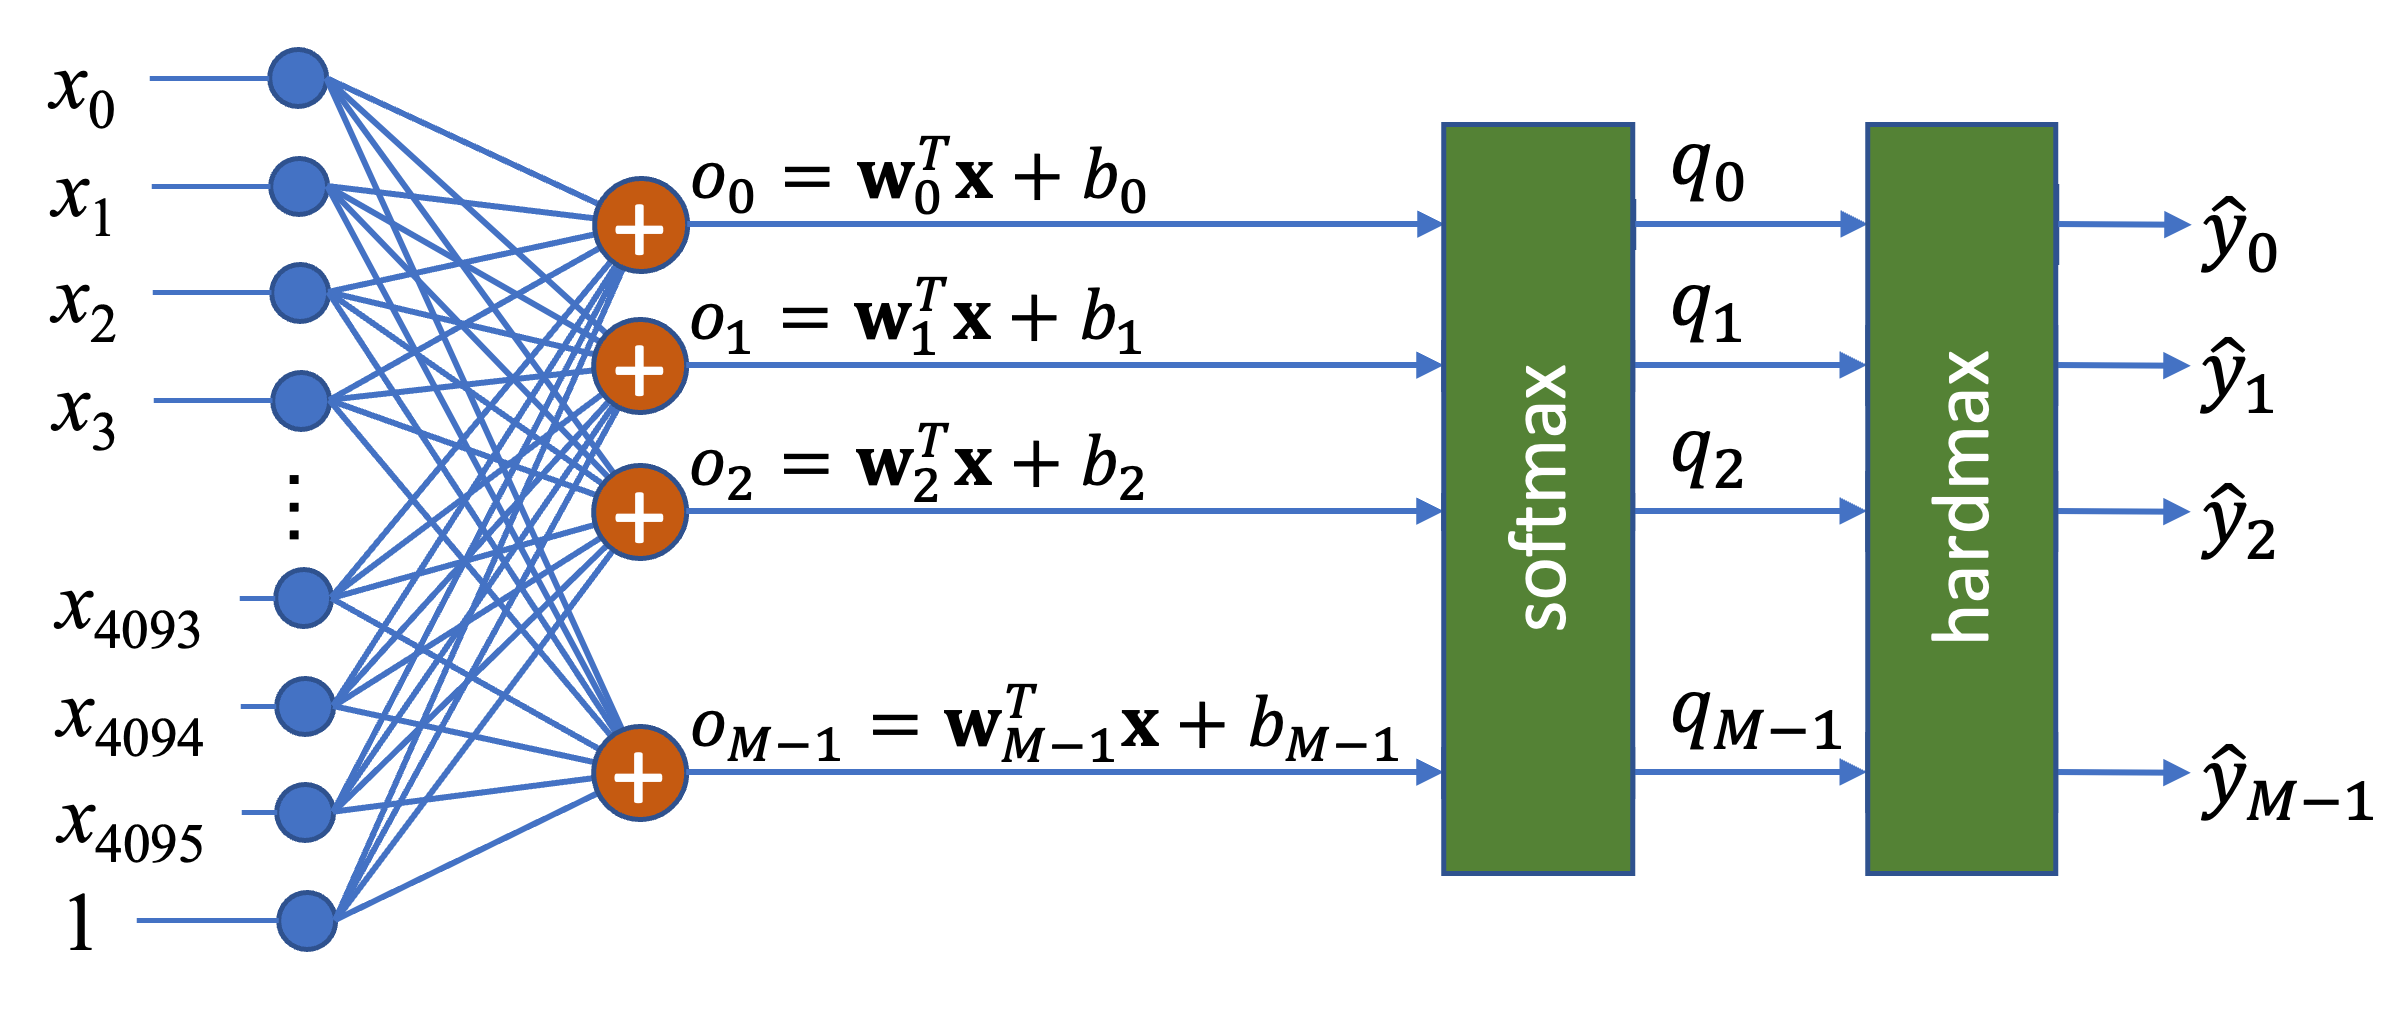
\includegraphics[width=\linewidth]{figs/SR_network.png}
\end{column}
\begin{column}{.38\textwidth}
\small
One-hot encoding of the label:
$$\vy = (0,\ldots,1,\ldots,0)^\intercal$$
One linear combination per class:
$$\vo = \vW\vx + \vb$$
\alert{Softmax} activation:
$$q_i = \frac{e^{o_i}}{\sum_j e^{o_j}}
  \;\Rightarrow\; q_i\in[0,1],\ \textstyle\sum_i q_i = 1$$
Class prediction: \texttt{hardmax}, i.e. $\arg\max_i q_i$.
\end{column}
\end{columns}
\end{frame}

\begin{frame}{The gradient has the same shape}
Cross entropy for $M$ classes: $\ \ell_\text{CE}(\vy,\vq) = -\sum_j y_j \log q_j$

\medskip
Working through the softmax Jacobian, everything collapses:
$$\frac{\partial \ell}{\partial \vW} = (\vq - \vy)\,\vx^\intercal
\qquad\qquad
\frac{\partial \ell}{\partial \vb} = \vq - \vy$$

\begin{keybox}[Same rule as before]
\textbf{error $\times$ input}, again. The messy Jacobian of the softmax cancels exactly
against the derivative of the cross entropy. This is not a coincidence: it is why this
pair of (activation, loss) is the standard choice.
\end{keybox}
\end{frame}

\begin{frame}[fragile]{A detail that bites in practice}
\begin{columns}[T]
\begin{column}{.48\textwidth}
\begin{lstlisting}
# overflows for large scores
def softmax(t):
    e = np.exp(t)
    return e / e.sum(axis=1, keepdims=True)
\end{lstlisting}
\end{column}
\begin{column}{.48\textwidth}
\begin{lstlisting}
# the constant cancels out
def softmax(t):
    e = np.exp(t - t.max(axis=1,
                         keepdims=True))
    return e / e.sum(axis=1, keepdims=True)
\end{lstlisting}
\end{column}
\end{columns}
\vspace{.6em}
$$\frac{e^{o_i}}{\sum_j e^{o_j}} = \frac{e^{o_i - c}}{\sum_j e^{o_j - c}}
  \quad \text{for any } c, \qquad \text{take } c = \max_j o_j$$
\begin{center}\small
Half of the numerical problems in deep learning are of this kind. Libraries do this for
you, which is one of the reasons to use them.
\end{center}
\end{frame}

\begin{frame}{Your turn}
\begin{practice}[Notebook DL1, section 3.2 \textbullet{} 12 minutes]
\begin{enumerate}
  \item Run the 10-class network on the digits dataset.
  \item \textbf{Exercise 3.} Explore epochs and learning rate.
  \item \textbf{Exercise 4.} Compute the \textbf{confusion matrix} on the validation set.
        Which digits get confused with which?
  \item \textbf{Exercise 5} (to discuss, no code): one 10-class network, or ten binary
        classifiers? What changes?
\end{enumerate}
\end{practice}
\end{frame}

%------------------------------------------------------------------ MLP
\begin{frame}{Multi-layer networks}
So far every model is \alert{linear}. We could apply a fixed non-linear transformation $\bm z = \bm f(\vx)$ first, as in
non-linear regression. But a \emph{fixed} transformation is a guess.

\medskip
\textbf{Better idea:} parametrize the transformation itself and learn it too. That is a
\alert{multi-layer perceptron}.

\vspace{-.3cm}

\begin{center}
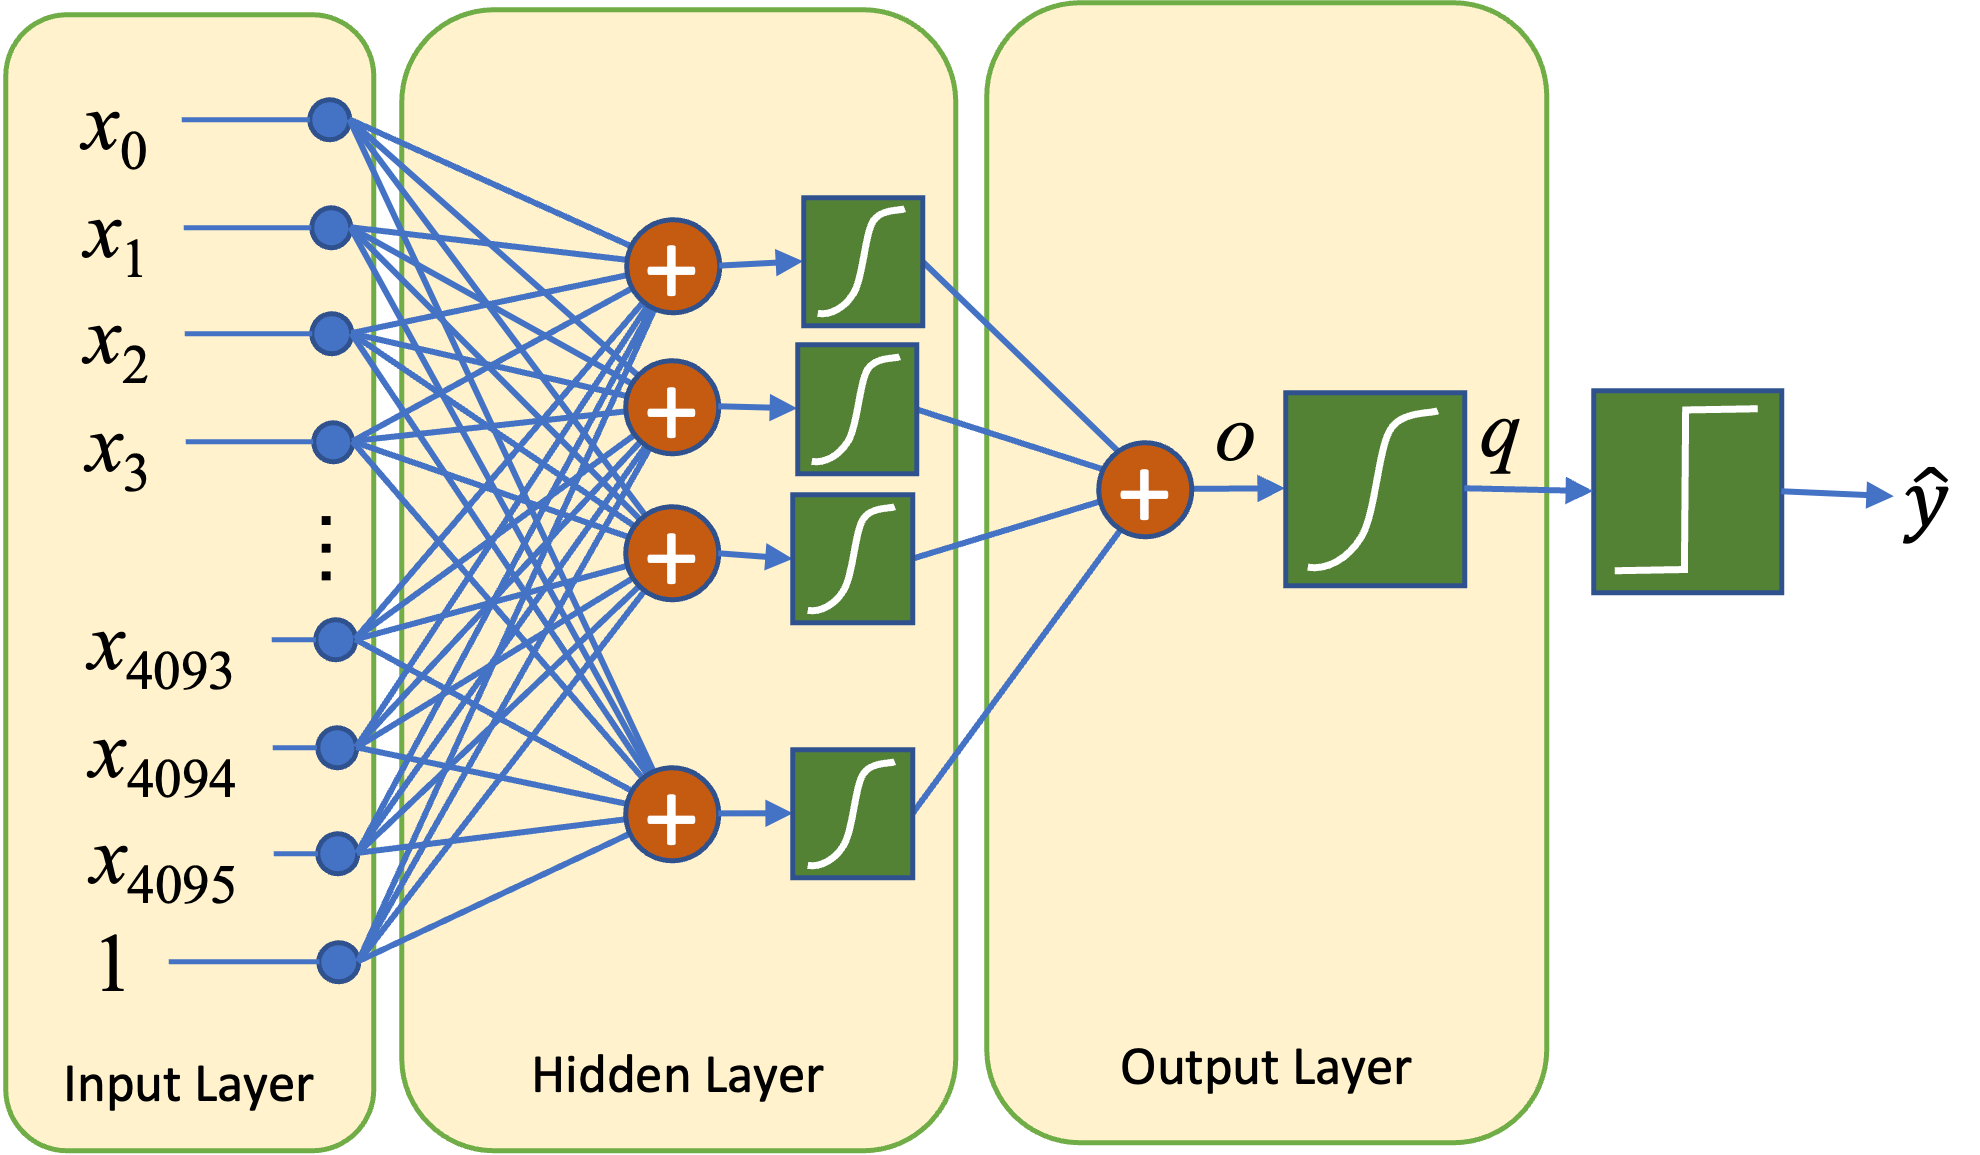
\includegraphics[height=.66\textheight]{figs/LR_MLPnetwork.png}
\end{center}
\end{frame}

\begin{frame}{Vocabulary and consequences}
\begin{itemize}
  \item Layers are counted ignoring the input layer; intermediate ones are
        \textbf{hidden layers}
  \item \textbf{Non-linear} activations are what makes the whole thing non-linear:
        stacking linear layers gives one linear layer
  \item This is already \textbf{deep learning}. Nothing else is needed, as long as the
        derivatives exist
  \item How many layers, how many neurons? \alert{Exploration}, guided by validation
  \item More data $\rightarrow$ more parameters you can afford
\end{itemize}
\end{frame}

\begin{frame}{A 2-layer network}
\centering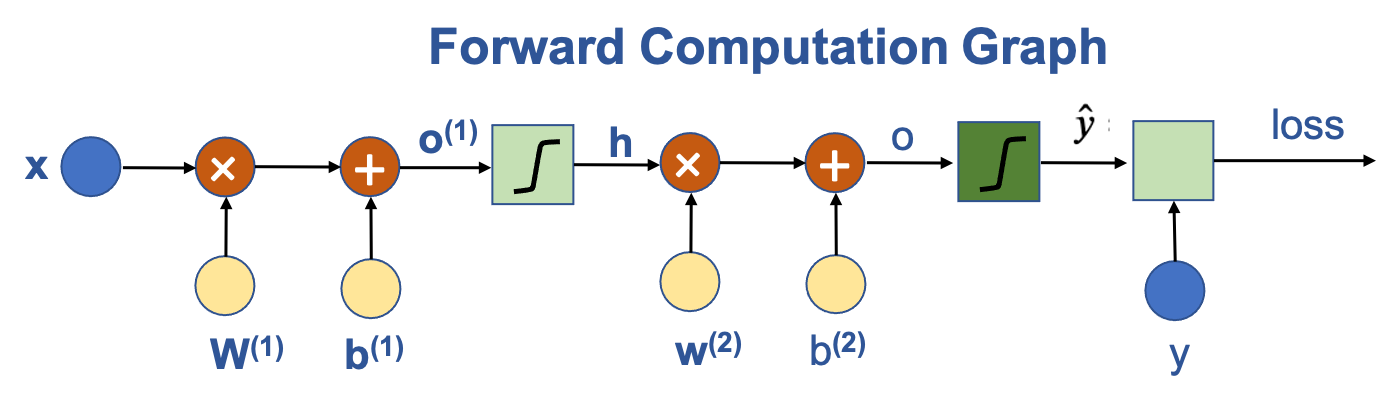
\includegraphics[width=.7\linewidth]{figs/forward_graph.png}
\begin{itemize}
  \item Hidden layer: $n_h$ units, $\tanh$ activation
  \item Output layer: one unit, logistic
  \item Loss: cross entropy
\end{itemize}
\begin{align*}
\vh &= \tanh\!\big(\vW^{(1)}\vx + \vb^{(1)}\big)\\
q  &= \text{logistic}\!\big({\vw^{(2)}}^\intercal \vh + b^{(2)}\big)
\end{align*}
\end{frame}

\begin{frame}{Back-propagation is the chain rule, read backwards}
\textbf{Output layer:} identical to before, with $\vh$ in the place of $\vx$
$$\frac{\partial \ell}{\partial \vw^{(2)}} = (q-y)\,\vh$$

\textbf{Hidden layer:} one more link in the chain
$$\frac{\partial \ell}{\partial \vW^{(1)}}
 = \underbrace{(q - y)}_{\text{output error}}
   \big[\underbrace{\vw^{(2)}}_{\text{how much each unit contributed}}
   \odot \underbrace{(\bm 1 - \vh^2)}_{\tanh'}\big]\vx^\intercal$$

\begin{keybox}[Why "backwards"]
The error computed at the output is \emph{propagated back}, multiplied at each step by the
weights of the layer and by the derivative of its activation. Each layer reuses the
quantity computed by the layer above it.
\end{keybox}
\end{frame}

\begin{comment}
\begin{frame}{A wrong gradient does not announce itself}
\begin{warnbox}[This version of the notebook fixes a real bug]
The previous version used $\;\partial \vh/\partial \vo^{(1)} = (\bm 1 - \vh)^2\;$ instead of
$\;\bm 1 - \vh^2$. The network still trained --- the sign was right --- but it was following
the wrong direction, which is why it needed a learning rate ten times smaller in the hidden
layer and diverged easily.
\end{warnbox}

\medskip
\textbf{The defence: numerical gradient checking.}
$$\frac{\partial \ell}{\partial w_{ij}} \;\approx\;
  \frac{\ell(w_{ij}+\epsilon) - \ell(w_{ij}-\epsilon)}{2\epsilon}$$
Compare with the analytical gradient: the relative error should be $\sim 10^{-9}$.
Cheap, and it catches what the loss curve hides.
\end{frame}
\end{comment}


\begin{frame}{Your turn}
\begin{practice}[Notebook DL1, section 3.3 \textbullet{} 12 minutes]
\begin{enumerate}
  \item Run the gradient check. Then break it on purpose: change \texttt{(1 - h**2)}
        back to \texttt{(1 - h)**2} and look at what the check reports, and at what the
        loss curve reports.
  \item Train the 2-layer network on both datasets.
  \item \textbf{Exercise 6.} Vary $n_h$, $\rho$ and the number of epochs. Find a divergent
        setting and explain it in terms of saturation.
  \item \textbf{Exercise 7} (if you have time): solve the same problems with
        \texttt{sklearn}'s \texttt{MLPClassifier}.
\end{enumerate}
\end{practice}
\end{frame}

%------------------------------------------------------------------ activations
\begin{frame}{The problem with saturating activations}
\begin{center}
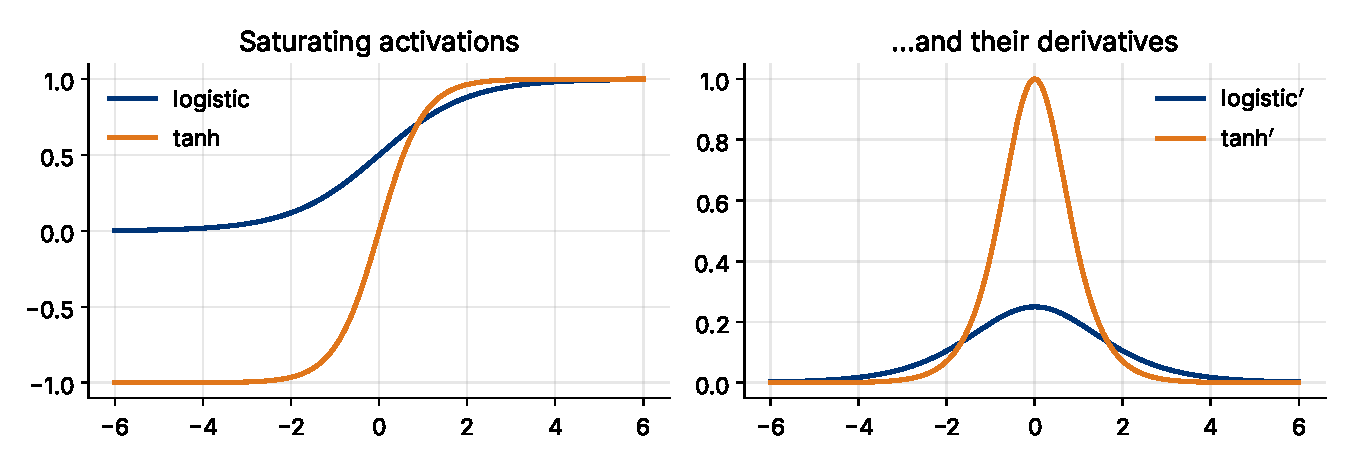
\includegraphics[width=.78\textwidth]{figs/saturation.pdf}
\end{center}
The derivative vanishes away from the origin. In a deep network these factors
\alert{multiply}: with a few layers, the gradient reaching the first layer is numerically
zero. This is the \textbf{vanishing gradient} problem.
\end{frame}

\begin{frame}{Activation functions used in practice}
\begin{center}
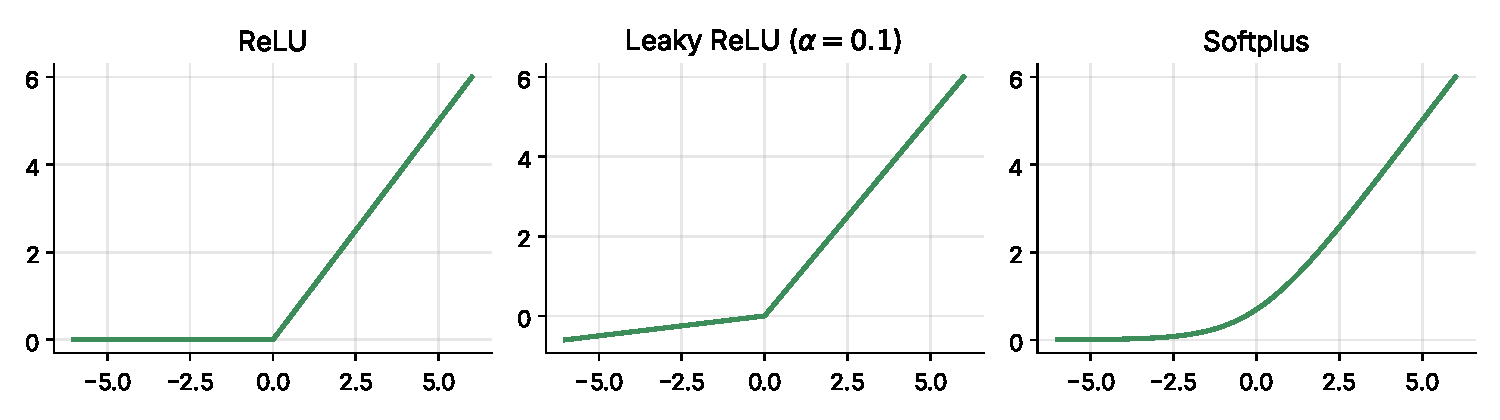
\includegraphics[width=.9\textwidth]{figs/activations.pdf}
\end{center}
\begin{itemize}\small
  \item \textbf{ReLU}: $\max(0,t)$. Derivative is a step. The default choice for hidden layers
  \item \textbf{Leaky ReLU / PReLU}: $\max(\alpha t, t)$, avoids exactly-zero derivatives
  \item \textbf{Softplus}: $\log(1+e^t)$, a smooth ReLU; its derivative is the logistic
\end{itemize}
Activations must be \emph{non-linear}; they need not be bounded or probabilistic --- except,
usually, at the output layer.
\end{frame}

\begin{frame}{And for regression?}
Two changes, nothing else:
\begin{itemize}
  \item \textbf{Linear} activation at the output unit (the target is not in $[0,1]$)
  \item \textbf{Square loss} instead of the cross entropy:
        $\ \ell(y,\hat y) = (y - \hat y)^2$
\end{itemize}
\vspace{.5em}
\begin{keybox}[Same machinery]
Topology, loss, forward, backward, update. Changing the task changes the last layer and
the loss; the rest of the network, and all of back-propagation, is untouched.
\end{keybox}
\end{frame}

\begin{frame}{Session 1 wrap-up}
\begin{columns}[T]
\begin{column}{.5\textwidth}
\textbf{What we built}
\begin{itemize}\small
  \item A single neuron $=$ logistic regression
  \item Softmax output for $M$ classes
  \item A hidden layer, and back-propagation
  \item Activation functions and why they matter
\end{itemize}
\end{column}
\begin{column}{.48\textwidth}
\textbf{What does not scale}
\begin{itemize}\small
  \item Deriving gradients by hand for each topology
  \item A wrong gradient is hard to detect
  \item Nothing here runs on a GPU
\end{itemize}
\end{column}
\end{columns}
\vspace{1em}
\begin{practice}[Before the next session]
Work through the two short official tutorials linked at the end of the notebook:
PyTorch \textbf{tensors} and \textbf{autograd}. 30 minutes, and session 2 will be much
easier.
\end{practice}
\end{frame}

%==============================================================================
\renewcommand{\sessiontag}{Session 2 \textbullet{} notebook DL2}
\section{Deep networks with PyTorch}

\begin{frame}{What PyTorch gives us}
\begin{columns}[T]
\begin{column}{.55\textwidth}
\begin{itemize}
  \item \textbf{Tensors}, numpy-like, that can live on a GPU
  \item \textbf{Automatic differentiation}: no more \texttt{backward} by hand
  \item \textbf{Pre-defined components}: layers, losses, optimizers, data loaders
  \item \textbf{Several levels of abstraction}, so you can drop down when you need to
\end{itemize}
\end{column}
\begin{column}{.42\textwidth}
\begin{keybox}[Today's plan]
\small
We rewrite \emph{the same model} four times, climbing one level of abstraction each time.

The point is not the final version: it is understanding what each level hides.
\end{keybox}
\end{column}
\end{columns}
\end{frame}

\begin{frame}[fragile]{Tensors}
\begin{columns}[T]
\begin{column}{.52\textwidth}
\begin{lstlisting}
import torch

x = torch.rand((100, 200))
t = torch.from_numpy(my_array)

x.size()          # shape
x.t()             # transpose
x.mm(x.t())       # matrix product
x.add(y)          # elementwise
x.add_(y)         # ... in place

x = x.to(device)  # move to the GPU
\end{lstlisting}
\end{column}
\begin{column}{.45\textwidth}
\begin{warnbox}[Two traps]
\small
\begin{itemize}
  \item \texttt{from\_numpy} \textbf{shares memory} with the array
  \item torch layers use \texttt{float32}; numpy defaults to \texttt{float64}.
        Mixing them is a very common error
\end{itemize}
\end{warnbox}
\end{column}
\end{columns}
\end{frame}

\begin{frame}[fragile]{Automatic differentiation}
\begin{columns}[T]
\begin{column}{.5\textwidth}
\begin{lstlisting}
x.requires_grad = True

y = (3 * torch.log(x)).sum()
y.backward()

x.grad        # == 3/x
\end{lstlisting}
\end{column}
\begin{column}{.47\textwidth}
\small
PyTorch records every operation on tensors with \texttt{requires\_grad} into a
\textbf{computation graph}. Calling \texttt{backward()} walks it backwards, applying the
chain rule --- exactly what we did by hand in session 1.
\end{column}
\end{columns}
\vspace{.5em}
\begin{warnbox}[Gradients accumulate]
A second \texttt{backward()} \alert{adds} to \texttt{.grad} instead of replacing it. This
is deliberate (it is useful), and it is why every training loop calls
\texttt{zero\_grad()}.
\end{warnbox}
\end{frame}

\begin{frame}{Your turn}
\begin{practice}[Notebook DL2, sections 1.2--1.3 \textbullet{} 10 minutes]
\begin{enumerate}
  \item Run the tensor and autograd cells.
  \item \textbf{Exercise 1}, the five steps: build a tensor from the data, take its square
        root, sum the squares, differentiate, and check the result by hand.
  \item Step 1.5 is the important one: make \texttt{backward()} runnable twice with the
        same result. \emph{Why does it fail the second time?}
\end{enumerate}
\end{practice}
\end{frame}

\begin{frame}[fragile]{Level 1 --- tensors and autograd only}
\begin{columns}[T]
\begin{column}{.56\textwidth}
\begin{lstlisting}
W = .1 * torch.randn(n_in, n_out)
W.requires_grad_()
b = torch.zeros(n_out, requires_grad=True)

for epoch in range(epochs):
    pred = model(W, b, X_train)
    loss = nll(y_train, pred)
    loss.backward()

    with torch.no_grad():
        W -= rho * W.grad
        b -= rho * b.grad
        W.grad.zero_()
        b.grad.zero_()
\end{lstlisting}
\end{column}
\begin{column}{.42\textwidth}
\small
Compared with session 1, exactly one thing disappeared: the \texttt{backward} function.

\medskip
\texttt{torch.no\_grad()} tells PyTorch not to record the weight update itself as part of
the graph.
\end{column}
\end{columns}
\end{frame}

\begin{frame}[fragile]{Levels 2 and 3 --- \texttt{nn.Module}, \texttt{nn.Linear}, losses}
\begin{columns}[T]
\begin{column}{.5\textwidth}
\begin{lstlisting}
class MyNet(nn.Module):
    def __init__(self, nin, nout):
        super().__init__()
        self.W = nn.Parameter(.1*torch.randn(nin, nout))
        self.b = nn.Parameter(torch.zeros(nout))

    def forward(self, x):
        return softmax(x.mm(self.W) + self.b)
\end{lstlisting}
\begin{lstlisting}
class MyNet(nn.Module):
    def __init__(self, nin, nout):
        super().__init__()
        self.lin = nn.Linear(nin, nout)

    def forward(self, x):
        return self.lin(x)

loss_func = nn.CrossEntropyLoss()
\end{lstlisting}
\end{column}
\begin{column}{.47\textwidth}
\small
\textbf{Level 2.} \texttt{nn.Parameter} registers a tensor as trainable; the loop becomes
\texttt{for p in net.parameters()}.

\medskip
\textbf{Level 3.} \texttt{nn.Linear} brings its own weights \emph{and} a sensible
initialization. \texttt{nn.CrossEntropyLoss} includes the softmax, so the network outputs
raw scores and takes integer labels, not one-hot.

\medskip
\alert{The faster convergence you will see is due to the initialization}, not to any
change in the model.
\end{column}
\end{columns}
\end{frame}

\begin{frame}[fragile]{Level 4 --- optimizers}
\begin{columns}[T]
\begin{column}{.5\textwidth}
\begin{lstlisting}
from torch import optim

opt = optim.SGD(net.parameters(), lr=0.1)

for epoch in range(epochs):
    pred = net(X_train)
    loss = loss_func(pred, y_train)
    loss.backward()
    opt.step()
    opt.zero_grad()
\end{lstlisting}
\end{column}
\begin{column}{.47\textwidth}
\small
The update rule is now a replaceable object: \texttt{SGD}, \texttt{Adam},
\texttt{RMSprop}, with momentum, schedulers, and so on.

\medskip
\texttt{opt.step()} applies the rule to every registered parameter;
\texttt{opt.zero\_grad()} clears the accumulated gradients.
\end{column}
\end{columns}
\vspace{.4em}
\begin{center}\small
Four levels, same model. From here on we only use the last one.
\end{center}
\end{frame}

\begin{frame}{Your turn}
\begin{practice}[Notebook DL2, sections 2.1--2.3 \textbullet{} 14 minutes]
\begin{enumerate}
  \item Run the four versions and check they give the same thing.
  \item \textbf{Exercise 2.} Replace SGD by \textbf{Adam}, and add a learning rate
        \textbf{scheduler} (\texttt{ExponentialLR}).
  \item Compare the curves. How many epochs does Adam need to reach what SGD reached?
\end{enumerate}
\end{practice}
\end{frame}

\begin{frame}[fragile]{Minibatches: from GD to SGD}
\begin{columns}[T]
\begin{column}{.45\textwidth}
\centering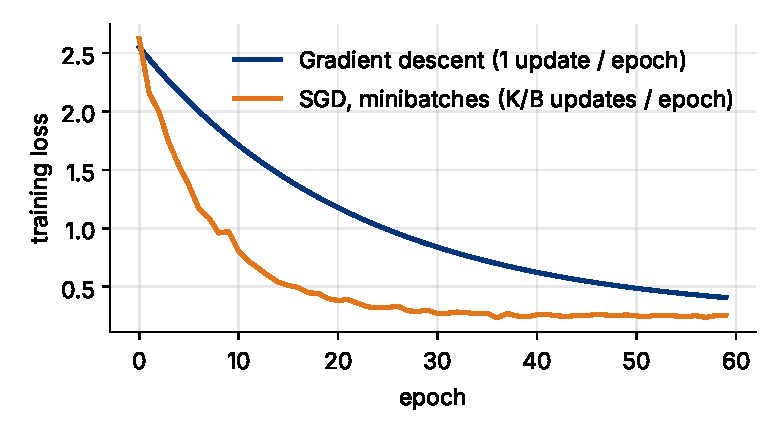
\includegraphics[width=\linewidth]{figs/gd_vs_sgd.pdf}
\end{column}
\begin{column}{.52\textwidth}
\small
Until now, one gradient over the \emph{whole} training set per epoch: one update per epoch.

\medskip
\textbf{SGD with minibatches}: split the epoch into batches of $B$ samples and update after
each one. With $K$ samples that is $K/B$ updates per epoch, each one noisier but almost as
useful.

\begin{lstlisting}
train_ds = TensorDataset(X_train, y_train)
train_dl = DataLoader(train_ds,
                      batch_size=64,
                      shuffle=True)

for xb, yb in train_dl:
    ...
\end{lstlisting}
\end{column}
\end{columns}
\end{frame}

\begin{frame}[fragile]{Multi-layer networks in five lines}
\begin{lstlisting}
my_net = nn.Sequential(
    nn.Linear(n_in, 200), nn.ReLU(),
    nn.Linear(200, 50),   nn.ReLU(),
    nn.Linear(50, 20),    nn.ReLU(),
    nn.Linear(20, n_out))
\end{lstlisting}
\vspace{.3em}
Compare with session 1: we derived the gradients of a \emph{two}-layer network over two
slides. This network has four, and we need not to differentiate anything.

\begin{practice}[Notebook DL2, sections 2.4--2.5 \textbullet{} 9 minutes]
Run the \texttt{DataLoader} version and the \texttt{nn.Sequential} network. Look at the
final accuracy, and then look at the \textbf{gap between the training and the validation
curves}. We will come back to that gap in a minute.
\end{practice}
\end{frame}

%------------------------------------------------------------------ generalization
\begin{frame}{Over-fitting, read from the curves}
\begin{columns}[T]
\begin{column}{.5\textwidth}
\textbf{What you should have seen}
\begin{itemize}\small
  \item training accuracy $\rightarrow$ 100\,\%
  \item validation accuracy saturates around 79\,\%
  \item the validation \emph{loss} stops going down and starts to \alert{grow}
\end{itemize}
\end{column}
\begin{column}{.48\textwidth}
\begin{keybox}[The two symptoms are different]
\small
Accuracy saturating = the model has learnt what it can.

Validation loss \emph{growing} = the model is becoming \alert{confidently wrong}.
\end{keybox}
\end{column}
\end{columns}
\vspace{.6em}
Cross-validation over every possible topology is hopeless: too many configurations.
In practice we combine it with techniques that \emph{limit} the effective capacity.
\end{frame}

\begin{frame}[fragile]{Penalty terms: L2 and L1}
$$R(\vw) + \lambda\|\vw\|^2 \qquad\qquad R(\vw) + \lambda\|\vw\|_1$$

\begin{lstlisting}
opt = optim.SGD(net.parameters(), lr=0.01, weight_decay=1e-2)
\end{lstlisting}

\begin{keybox}[What to expect on our dataset]
\small
Accuracy barely moves ($0.792 \rightarrow 0.792$), but the validation loss at the end of
training drops from $1.08$ to $0.79$.

\medskip
The regularized network does not make fewer mistakes: it makes them \emph{less
confidently}. Which of the two numbers matters is a decision about your problem, not about
the method.
\end{keybox}
\end{frame}

\begin{frame}[fragile]{Dropout}
\begin{columns}[T]
\begin{column}{.46\textwidth}
\centering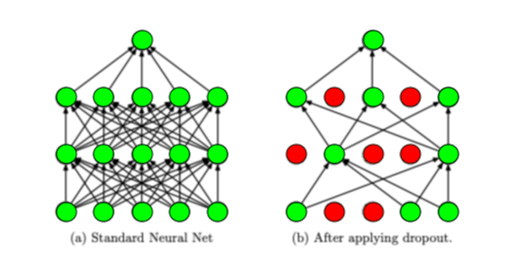
\includegraphics[width=\linewidth]{figs/dropout.png}
\end{column}
\begin{column}{.5\textwidth}
\begin{lstlisting}
nn.Sequential(
    nn.Linear(n_in, 200), nn.ReLU(), nn.Dropout(0.5),
    nn.Linear(200, 50),   nn.ReLU(), nn.Dropout(0.5),
    nn.Linear(50, 20),    nn.ReLU(),
    nn.Linear(20, n_out))
\end{lstlisting}
\small
A fraction $p$ of the units is switched off at random \textbf{at each training step}. No
unit can rely on any other being present.

\medskip
At \emph{inference} time dropout is off and all units are used.
\end{column}
\end{columns}
\vspace{.3em}
\begin{warnbox}[The classic bug]
\texttt{net.train()} and \texttt{net.eval()} switch that behaviour. Evaluating without
\texttt{eval()} gives you random predictions.
\end{warnbox}
\end{frame}

\begin{frame}{Early stopping, done properly}
\begin{columns}[T]
\begin{column}{.52\textwidth}
\begin{itemize}\small
  \item Monitor the validation metric at every epoch
  \item Keep a copy of the \alert{best} model, not the last one
  \item Do not stop at the first bad epoch: wait \textbf{patience} epochs without
        improvement
\end{itemize}
\end{column}
\begin{column}{.46\textwidth}
\begin{keybox}[On our data]
\small
Monitoring the \textbf{loss} selects epoch $\approx 139$, with accuracy $0.760$.

The best \textbf{accuracy}, $0.792$, happens much later.
\end{keybox}
\end{column}
\end{columns}
\vspace{.6em}
\begin{center}
\alert{The criterion you monitor is the model you get.} Choose it on purpose.
\end{center}
\end{frame}

\begin{frame}{Your turn}
\begin{practice}[Notebook DL2, section 3 \textbullet{} 8 minutes in class, finish at home]
\begin{enumerate}
  \item Run the three experiments: weight decay, dropout, early stopping.
  \item \textbf{Exercise 3.} Sweep \texttt{weight\_decay} from $10^{-5}$ to $10^{-1}$.
  \item \textbf{Exercise 4.} Sweep the dropout probability. Note that the \emph{training}
        accuracy gets worse --- and that this is not a failure.
  \item \textbf{Exercise 5.} Combine the three. Is the combination better than the best one
        alone?
  \item Switch early stopping to \texttt{monitor='accuracy'} and see which model it picks.
\end{enumerate}
\end{practice}
\end{frame}

\begin{frame}{Session 2 wrap-up}
\begin{columns}[T]
\begin{column}{.5\textwidth}
\textbf{The ladder}
\begin{enumerate}\small
  \item tensors $+$ autograd
  \item \texttt{nn.Module} / \texttt{nn.Parameter}
  \item \texttt{nn.Linear} / \texttt{nn.CrossEntropyLoss}
  \item \texttt{torch.optim}, \texttt{DataLoader}, \texttt{nn.Sequential}
\end{enumerate}
\end{column}
\begin{column}{.48\textwidth}
\textbf{Controlling over-fitting}
\begin{itemize}\small
  \item weight decay (L2)
  \item dropout
  \item early stopping
  \item data augmentation $\rightarrow$ next session
\end{itemize}
\end{column}
\end{columns}
\vspace{.8em}
\begin{center}
Still missing: every model so far sees an image as 4096 unrelated numbers.
\end{center}
\end{frame}

%==============================================================================
\renewcommand{\sessiontag}{Session 3 \textbullet{} notebook DL3}
\section{Convolutional networks}

\begin{frame}{The convolution operator}
\begin{center}
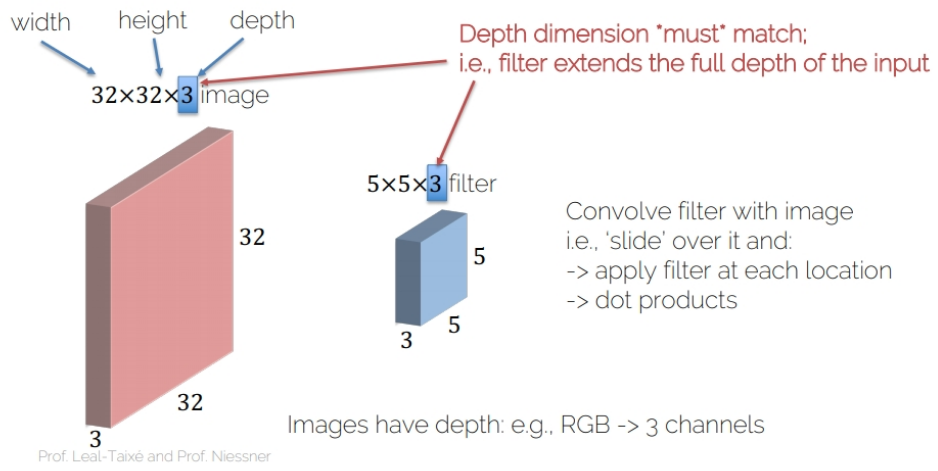
\includegraphics[height=.62\textheight]{figs/cnn01_convolutions_png.png}
\end{center}
A small \textbf{kernel} slides over the input; at each position we compute a weighted sum.
The kernel weights are the parameters, and they are the same at every position.
\end{frame}

\begin{frame}{Activation maps}
\begin{center}
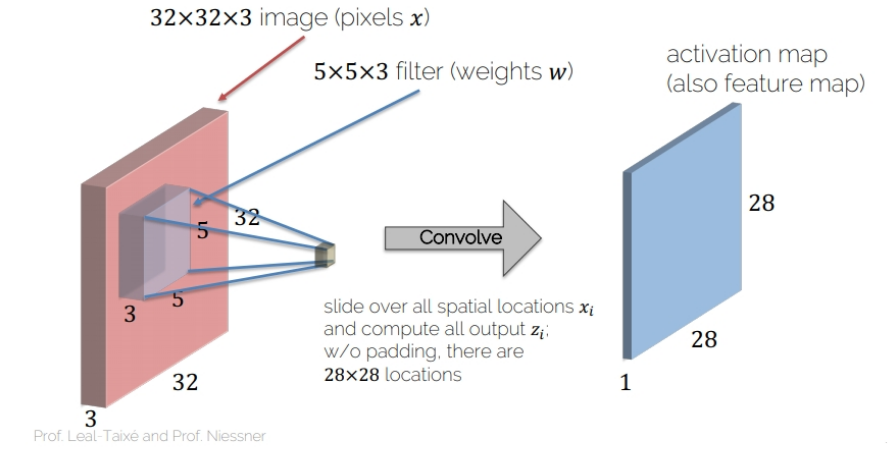
\includegraphics[height=.58\textheight]{figs/cnn03_act_map_png.png}
\end{center}
Each filter produces one \textbf{activation map} (a channel). A layer with $F$ filters
turns a $C\times H\times W$ input into an $F\times H'\times W'$ output.
\end{frame}

\begin{frame}{Why a dense layer is the wrong tool for an image}
\begin{columns}[T]
\begin{column}{.48\textwidth}
\centering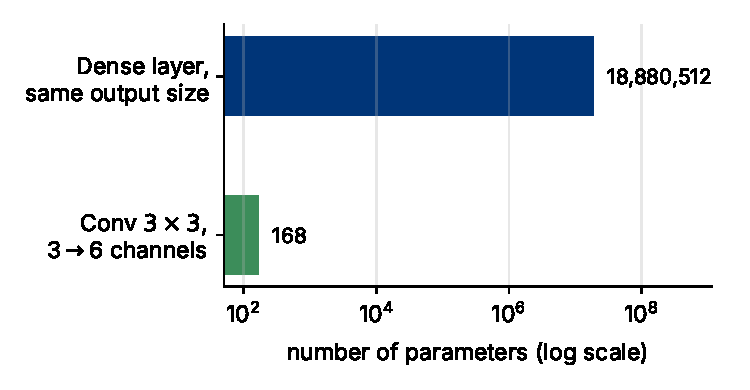
\includegraphics[width=\linewidth]{figs/params.pdf}
\end{column}
\begin{column}{.5\textwidth}
\begin{itemize}\small
  \item Do we really need every output to depend on every pixel?
  \item A dense layer has an enormous number of parameters: expensive, and prone to
        over-fitting
  \item And it is not \emph{translation invariant}: an edge in the top-left corner and the
        same edge in the centre are learnt separately
\end{itemize}
\begin{keybox}[The two ideas of a CNN]
\small
\textbf{Local connectivity}: each unit sees a small window.\\
\textbf{Weight sharing}: the same window is applied everywhere.
\end{keybox}
\end{column}
\end{columns}
\end{frame}

\begin{frame}[fragile]{Number of parameters of the convolutional layer}
\begin{lstlisting}
conv = nn.Conv2d(in_channels=3, out_channels=6, kernel_size=3,
                 stride=1, padding=1)
\end{lstlisting}
$$H' = \left\lfloor \frac{H + 2\,\text{padding} - \text{kernel}}{\text{stride}} \right\rfloor + 1$$
\begin{itemize}\small
  \item \texttt{padding=1} with \texttt{kernel=3} and \texttt{stride=1} \;$\Rightarrow$\;
        the spatial size is preserved
  \item \texttt{stride=2} halves it
  \item the number of channels is \texttt{out\_channels}, and has nothing to do with the
        spatial size
  \item parameters: $\text{out}\times\text{in}\times k \times k + \text{out}$, independent
        of the image size
\end{itemize}
\end{frame}

\begin{frame}{Pooling}
\begin{columns}[T]
\begin{column}{.5\textwidth}
\centering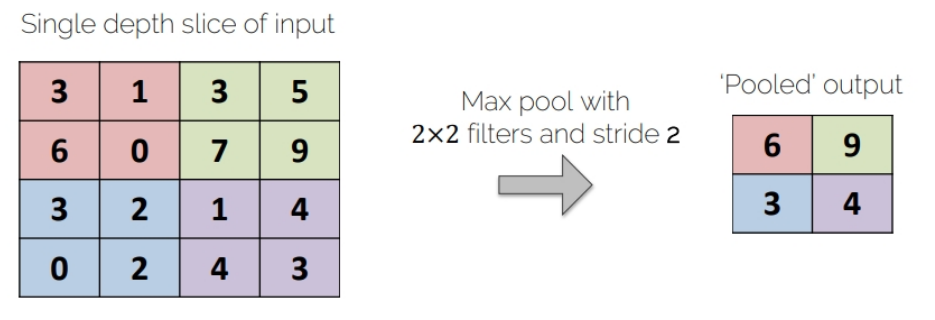
\includegraphics[width=\linewidth]{figs/cnn05_maxpool_png.png}
\end{column}
\begin{column}{.47\textwidth}
\small
Pooling \textbf{downsamples} the activation maps, combining a window of inputs into a
single output:
\begin{itemize}
  \item \texttt{nn.MaxPool2d(2)}: the maximum
  \item \texttt{nn.AvgPool2d(2)}: the average
\end{itemize}
It reduces the spatial size (and the computation that follows), and it gives a small
amount of invariance to translation.

\medskip
It has \textbf{no parameters}.
\end{column}
\end{columns}
\end{frame}

\begin{frame}{Your turn}
\begin{practice}[Notebook DL3, section 2 \textbullet{} 12 minutes]
\begin{enumerate}
  \item Load CIFAR10 and look at the images. \alert{Use a GPU runtime}
        (Runtime $\rightarrow$ Change runtime type).
  \item Apply the convolution and the two pooling operators, and check the shapes.
  \item Compare the parameter count of the convolution with that of an equivalent dense
        layer.
  \item \textbf{Exercise 1.} Predict, \emph{before running}, the output size with
        \texttt{padding=0}, with \texttt{stride=2}, and with \texttt{kernel\_size=5}.
\end{enumerate}
\end{practice}
\end{frame}

\begin{frame}[fragile]{A complete CNN}
\begin{columns}[T]
\begin{column}{.56\textwidth}
\begin{lstlisting}
class Net(nn.Module):
    def __init__(self):
        super().__init__()
        self.conv1 = nn.Conv2d(3, 5, 3, padding=1)
        self.conv2 = nn.Conv2d(5, 10, 3, padding=1)
        self.relu = nn.ReLU(inplace=True)
        self.pool = nn.MaxPool2d(2, 2)
        self.fc = nn.Linear(10*8*8, 10)

    def forward(self, x):
        x = self.pool(self.relu(self.conv1(x)))
        x = self.pool(self.relu(self.conv2(x)))
        x = torch.flatten(x, 1)
        return self.fc(x)
\end{lstlisting}
\end{column}
\begin{column}{.42\textwidth}
\small
$3\times32\times32$
$\rightarrow 5\times32\times32$
$\rightarrow 5\times16\times16$
$\rightarrow 10\times16\times16$
$\rightarrow 10\times8\times8$
$\rightarrow 640 \rightarrow 10$

\medskip
\textbf{Convolutional part} extracts features, \textbf{dense part} classifies them. This is
the standard shape of an image classifier.

\medskip
The training loop is \emph{exactly} the one from session 2.
\end{column}
\end{columns}
\end{frame}

\begin{frame}{Your turn}
\begin{practice}[Notebook DL3, section 3 \textbullet{} 15 minutes]
\begin{enumerate}
  \item Train the CNN for 10 epochs and look at the curves and at the \textbf{per-class}
        accuracy. Which classes are hard? Does that make sense?
  \item \textbf{Exercise 2.} Make the network bigger: more filters (16 and 32), a third
        convolutional block, a hidden dense layer. Which change buys the most accuracy per
        added parameter?
\end{enumerate}
\vspace{.2em}
While it trains: compare the number of parameters of this CNN with a dense network on the
same input.
\end{practice}
\end{frame}

\begin{frame}[fragile]{Data augmentation}
\begin{columns}[T]
\begin{column}{.52\textwidth}
\begin{lstlisting}
transform_augmented = transforms.Compose([
    transforms.RandomHorizontalFlip(),
    transforms.RandomCrop(32, padding=4),
    transforms.ToTensor(),
    transforms.Normalize(mean, std)])
\end{lstlisting}
\end{column}
\begin{column}{.45\textwidth}
\small
Random transformations that \textbf{do not change the label}: a mirrored cat is a cat.

\medskip
Applied \emph{on the fly}, differently at each epoch, and only to the \textbf{training}
set.
\end{column}
\end{columns}
\vspace{.4em}
\begin{warnbox}[Which transformations are valid is a modelling decision]
A vertical flip is fine for satellite images and wrong for street photos. For handwritten
digits, a horizontal flip turns a 2 into something that is not a 2 --- and rotating a 6 far
enough gives a 9.
\end{warnbox}
\end{frame}

\begin{frame}{Transfer learning}
\begin{columns}[T]
\begin{column}{.52\textwidth}
\begin{enumerate}\small
  \item Take a network trained on a much larger dataset (ResNet18 on ImageNet)
  \item \textbf{Freeze} the convolutional backbone: it already knows how to extract
        general image features
  \item Replace the last layer with one that has our number of classes
  \item Train \emph{only} that layer
\end{enumerate}
\end{column}
\begin{column}{.45\textwidth}
\begin{keybox}[The numbers]
\small
ResNet18: $\approx 11.2$M parameters.\\
Trainable after freezing: $5130$, i.e. $0.05\,\%$.

\medskip
And it beats, on a tenth of the data, a CNN trained from scratch on all of it.
\end{keybox}
\end{column}
\end{columns}
\vspace{.5em}
\begin{center}\small
On any image problem with a small dataset, this is the first thing to try.
\end{center}
\end{frame}

\begin{frame}[fragile]{Transfer learning in code}
\begin{lstlisting}
self.resnet = models.resnet18(weights=models.ResNet18_Weights.DEFAULT)

for p in self.resnet.parameters():      # freeze the ResNet weights
    p.requires_grad = False

self.resnet.fc = nn.Linear(self.resnet.fc.in_features, 10)   # new head
\end{lstlisting}
\begin{itemize}\small
  \item The pretrained network expects \textbf{its} input size and normalization
        ($224\times224$, ImageNet statistics)
  \item The new layer is created with \texttt{requires\_grad=True}, so it is the only one
        that trains
  \item \textbf{Fine-tuning}: unfreeze the backbone afterwards and continue with a much
        smaller learning rate
\end{itemize}
\end{frame}

\begin{frame}{Your turn}
\begin{practice}[Notebook DL3, sections 4--5 \textbullet{} 15 minutes]
\begin{enumerate}
  \item Train the same CNN with \textbf{data augmentation} and compare.
        \textbf{Exercise 3}: try more epochs, and other transformations.
  \item Run the \textbf{transfer learning} section. Compare the accuracy, and the number
        of trainable parameters, with the CNN trained from scratch.
  \item \textbf{Exercise 4.} Unfreeze the backbone and fine-tune with a small learning
        rate. Does it help? What does it cost?
\end{enumerate}
\end{practice}
\end{frame}

\begin{frame}{Where this block leaves you}
\begin{itemize}
  \item A neural network is a \textbf{topology}, a \textbf{loss} and an
        \textbf{optimization rule}; back-propagation is the chain rule applied backwards
  \item A library removes the gradients from your hands and gives you optimizers, data
        loaders and regularization layers --- but the bugs move to \texttt{train()/eval()},
        to dtypes and to shapes
  \item A \textbf{convolutional} topology encodes locality and weight sharing, with orders
        of magnitude fewer parameters
  \item Most practical image problems start from a \textbf{pretrained} network
\end{itemize}
\vspace{.5em}
\begin{keybox}[Next]
The same ideas, applied to text: embeddings, and the topologies built on top of them.
\end{keybox}
\end{frame}

\end{document}
